\documentclass[tikz, 11pt]{standalone}
%
\usetikzlibrary{calc}
\usepackage{graphicx}
\usepackage[scaled=0.92]{helvet}%3.75
\renewcommand{\familydefault}{\sfdefault}
\usepackage{textcomp}
%
\graphicspath{{Cropped/}}
%
\newlength{\PicWidth}
\newlength{\VSep}
\newlength{\HSep}
\newlength{\LabelSep}
%
\begin{document}
	%	
	\setlength{\PicWidth}{2.8cm}
	\setlength{\VSep}{1ex}
	\setlength{\HSep}{1.5ex}
	\setlength{\LabelSep}{0.5ex}
	%	
	\scriptsize % font size
	%
	\begin{tikzpicture}[every node/.style={inner sep=0ex},%
						MediaLabel/.style={font={\bfseries}, align=left}]
		%
		% YPD
		\path (0,0) node (YPD) {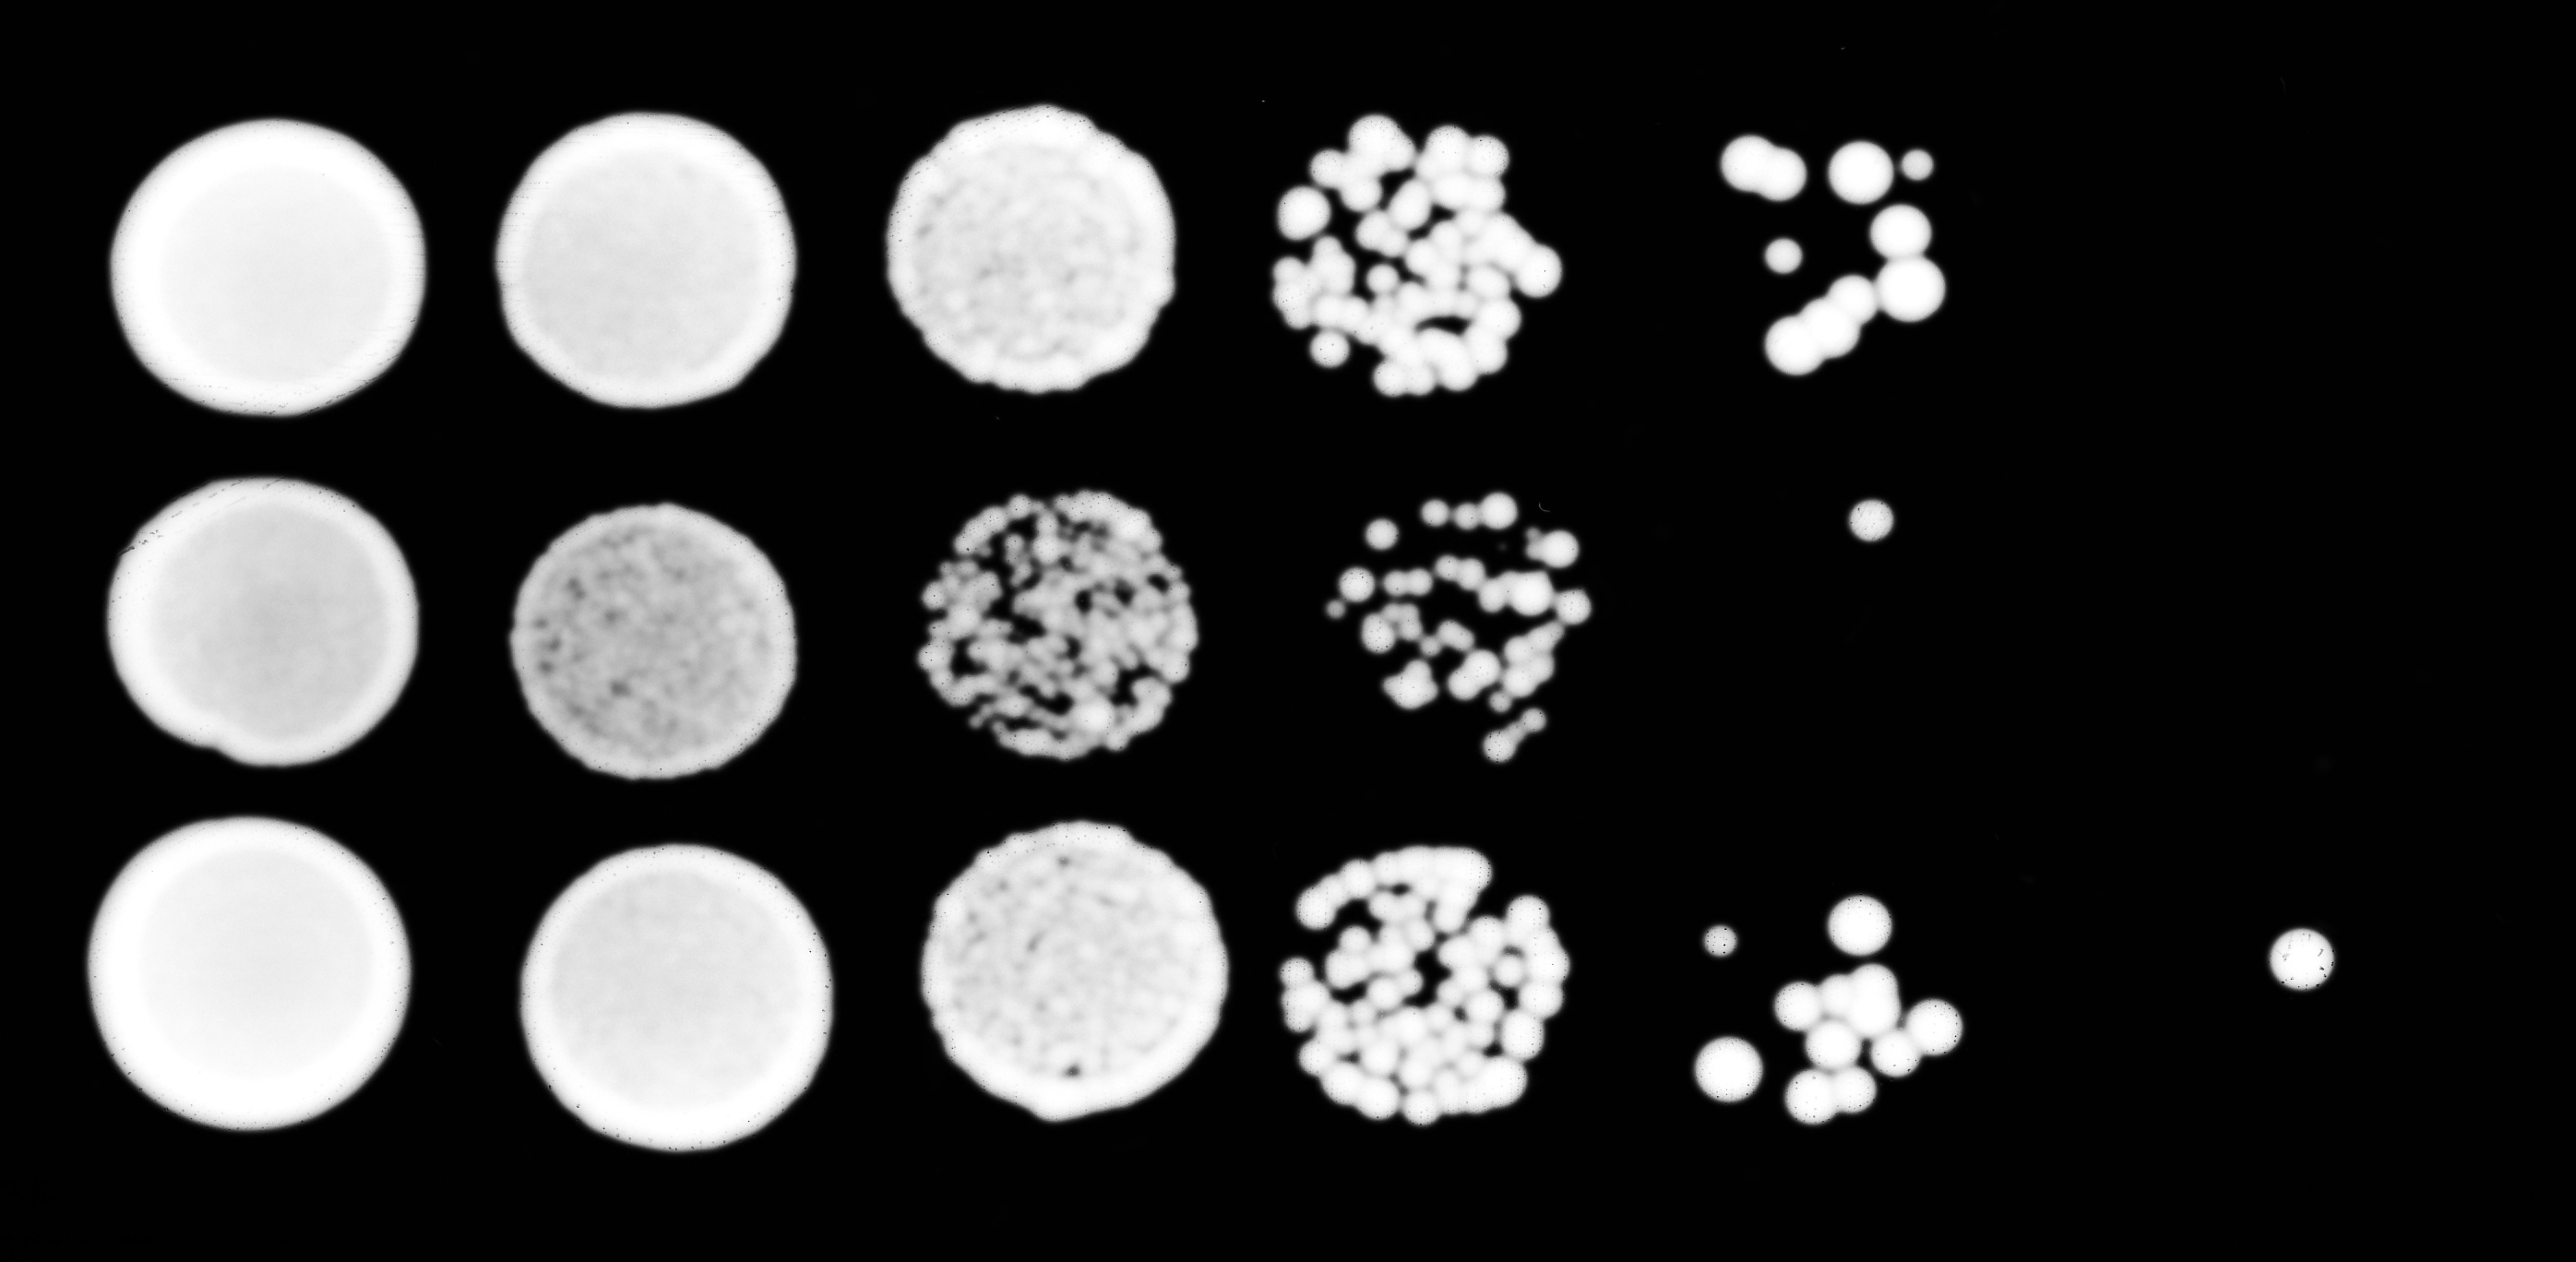
\includegraphics[width=\PicWidth]{YPD_DMSO.jpg}};
		% strains
		\pgfmathsetmacro{\Start}{0.22}
		\pgfmathsetmacro{\Sep}{0.28}
		\foreach[count=\i] \strain in {WT, \textit{arp8$\Delta$}, \textit{ino80-aa}}{
			\pgfmathsetmacro{\x}{\Start+(\i-1)*\Sep}
			\path ($(YPD.north west)!\x!(YPD.south west)$) node[xshift=-\LabelSep, anchor=east] {\strain};
		}
		%
		% SC_wo_I
		\path (YPD.south) ++(0,-\VSep) node[anchor=north] (SC_wo_I) {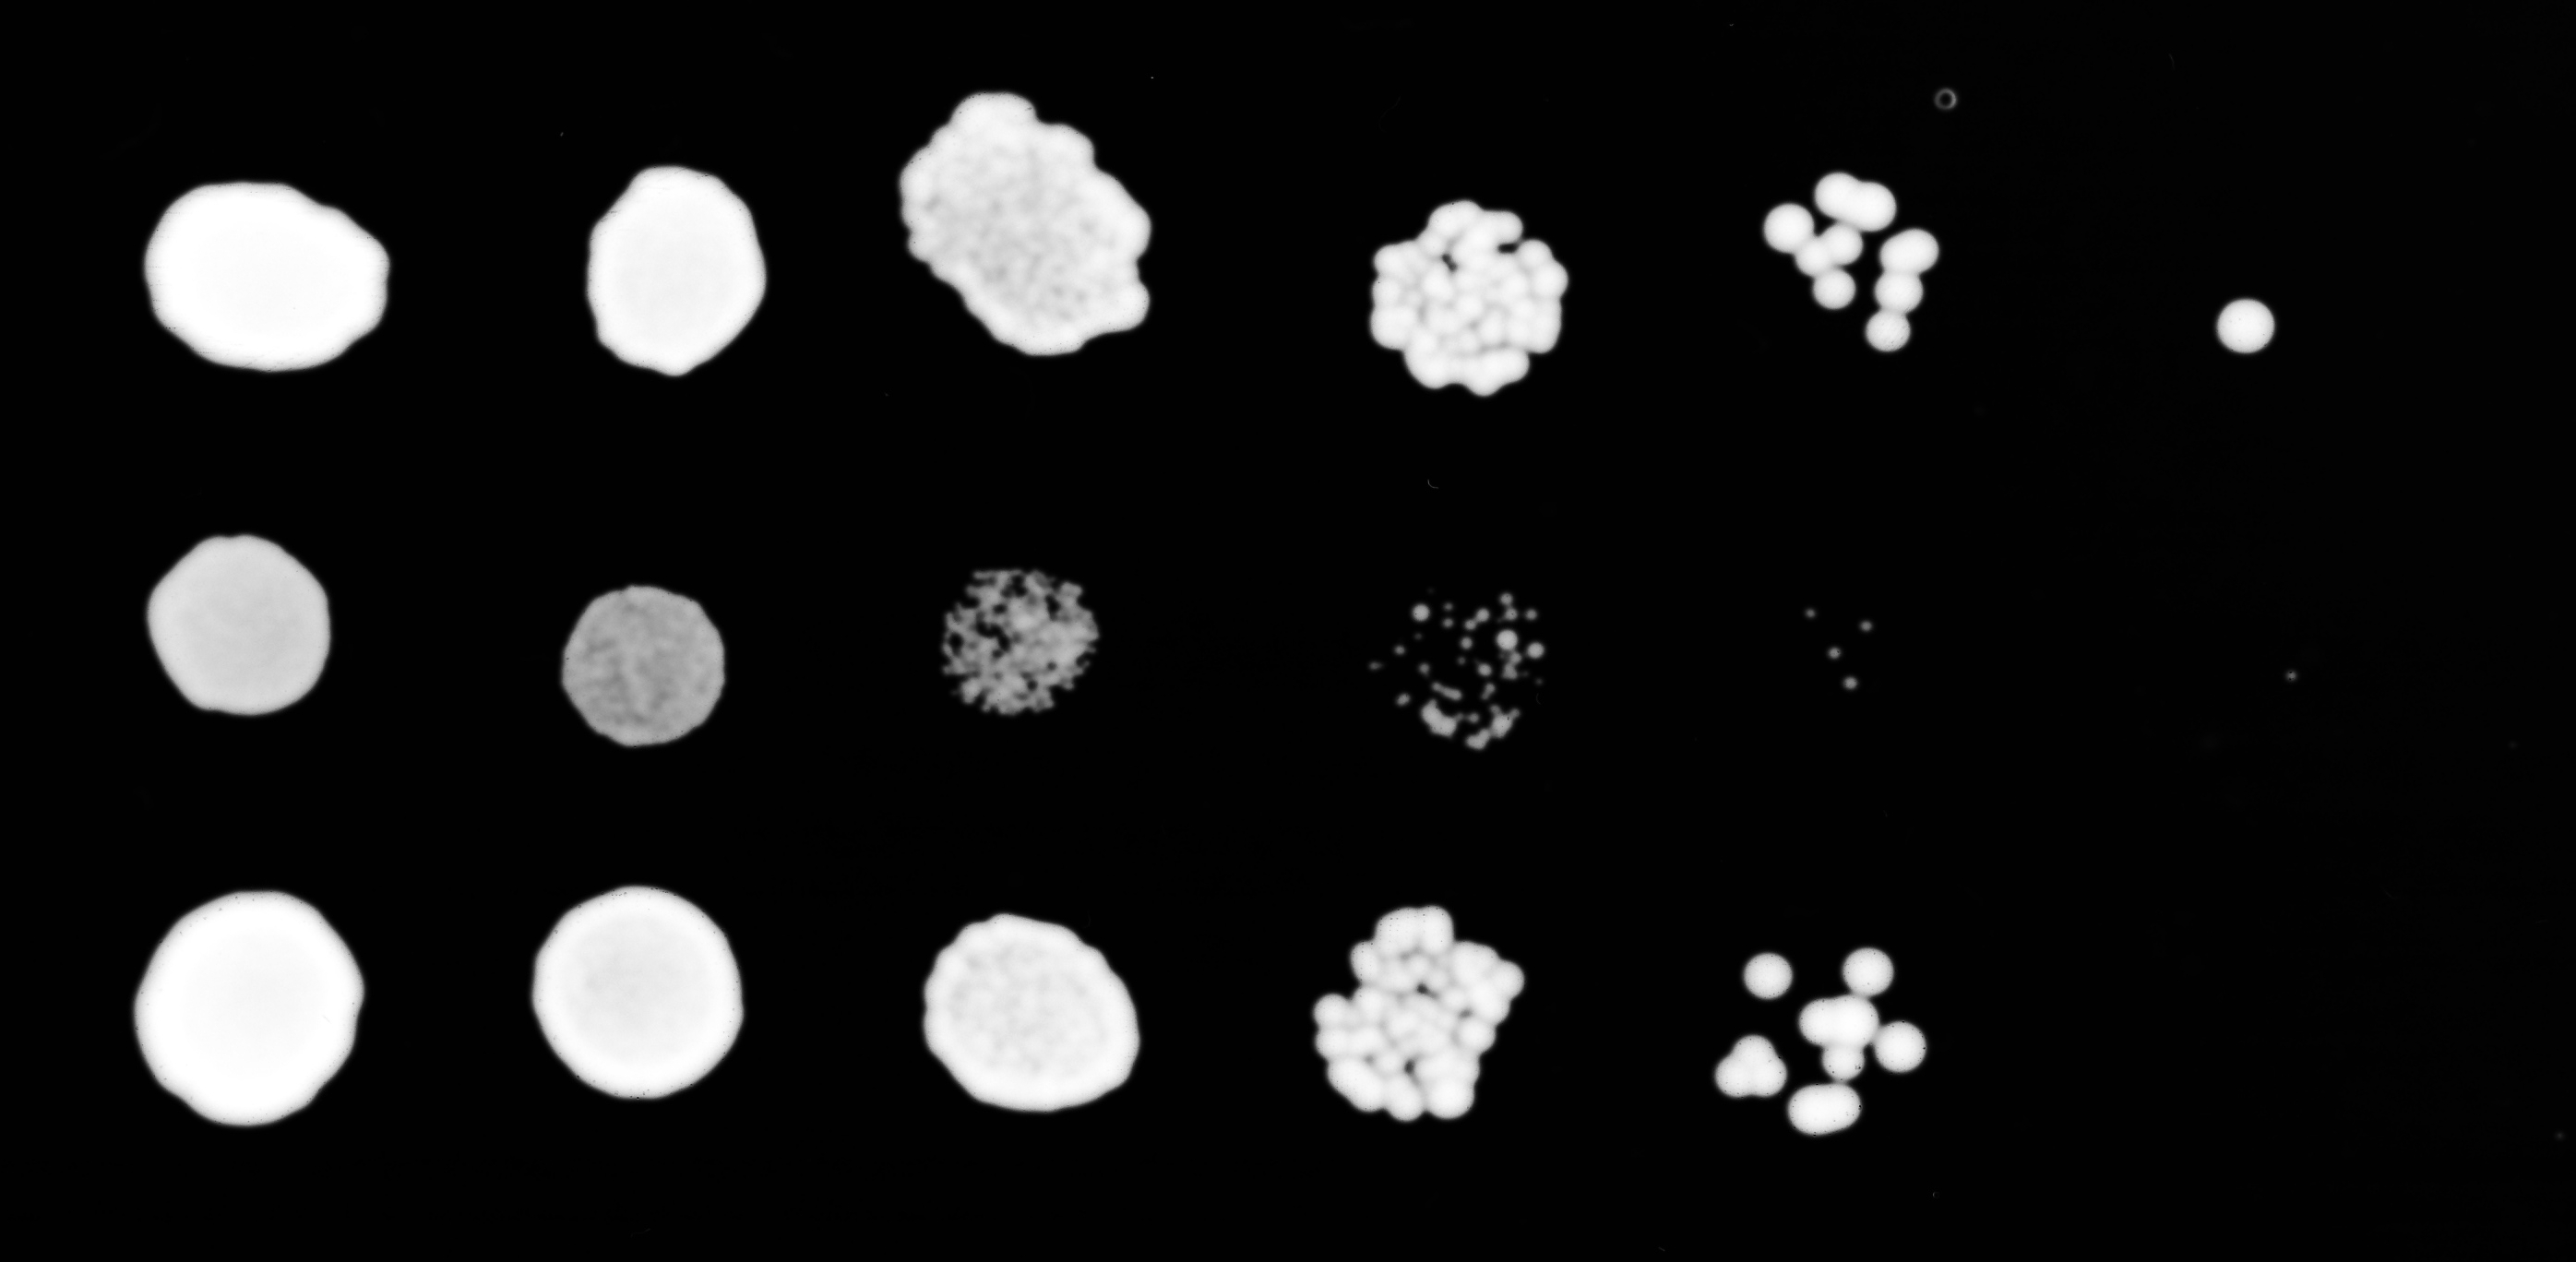
\includegraphics[width=\PicWidth]{SC_wo_I_DMSO.jpg}};
		% strains
		\pgfmathsetmacro{\Start}{0.22}
		\pgfmathsetmacro{\Sep}{0.28}
		\foreach[count=\i] \strain in {WT, \textit{arp8$\Delta$}, \textit{ino80-aa}}{
			\pgfmathsetmacro{\x}{\Start+(\i-1)*\Sep}
			\path ($(SC_wo_I.north west)!\x!(SC_wo_I.south west)$) node[xshift=-\LabelSep, anchor=east] {\strain};
		}
		%
		% YPE
		\path (SC_wo_I.south) ++(0,-\VSep) node[anchor=north] (YPE) {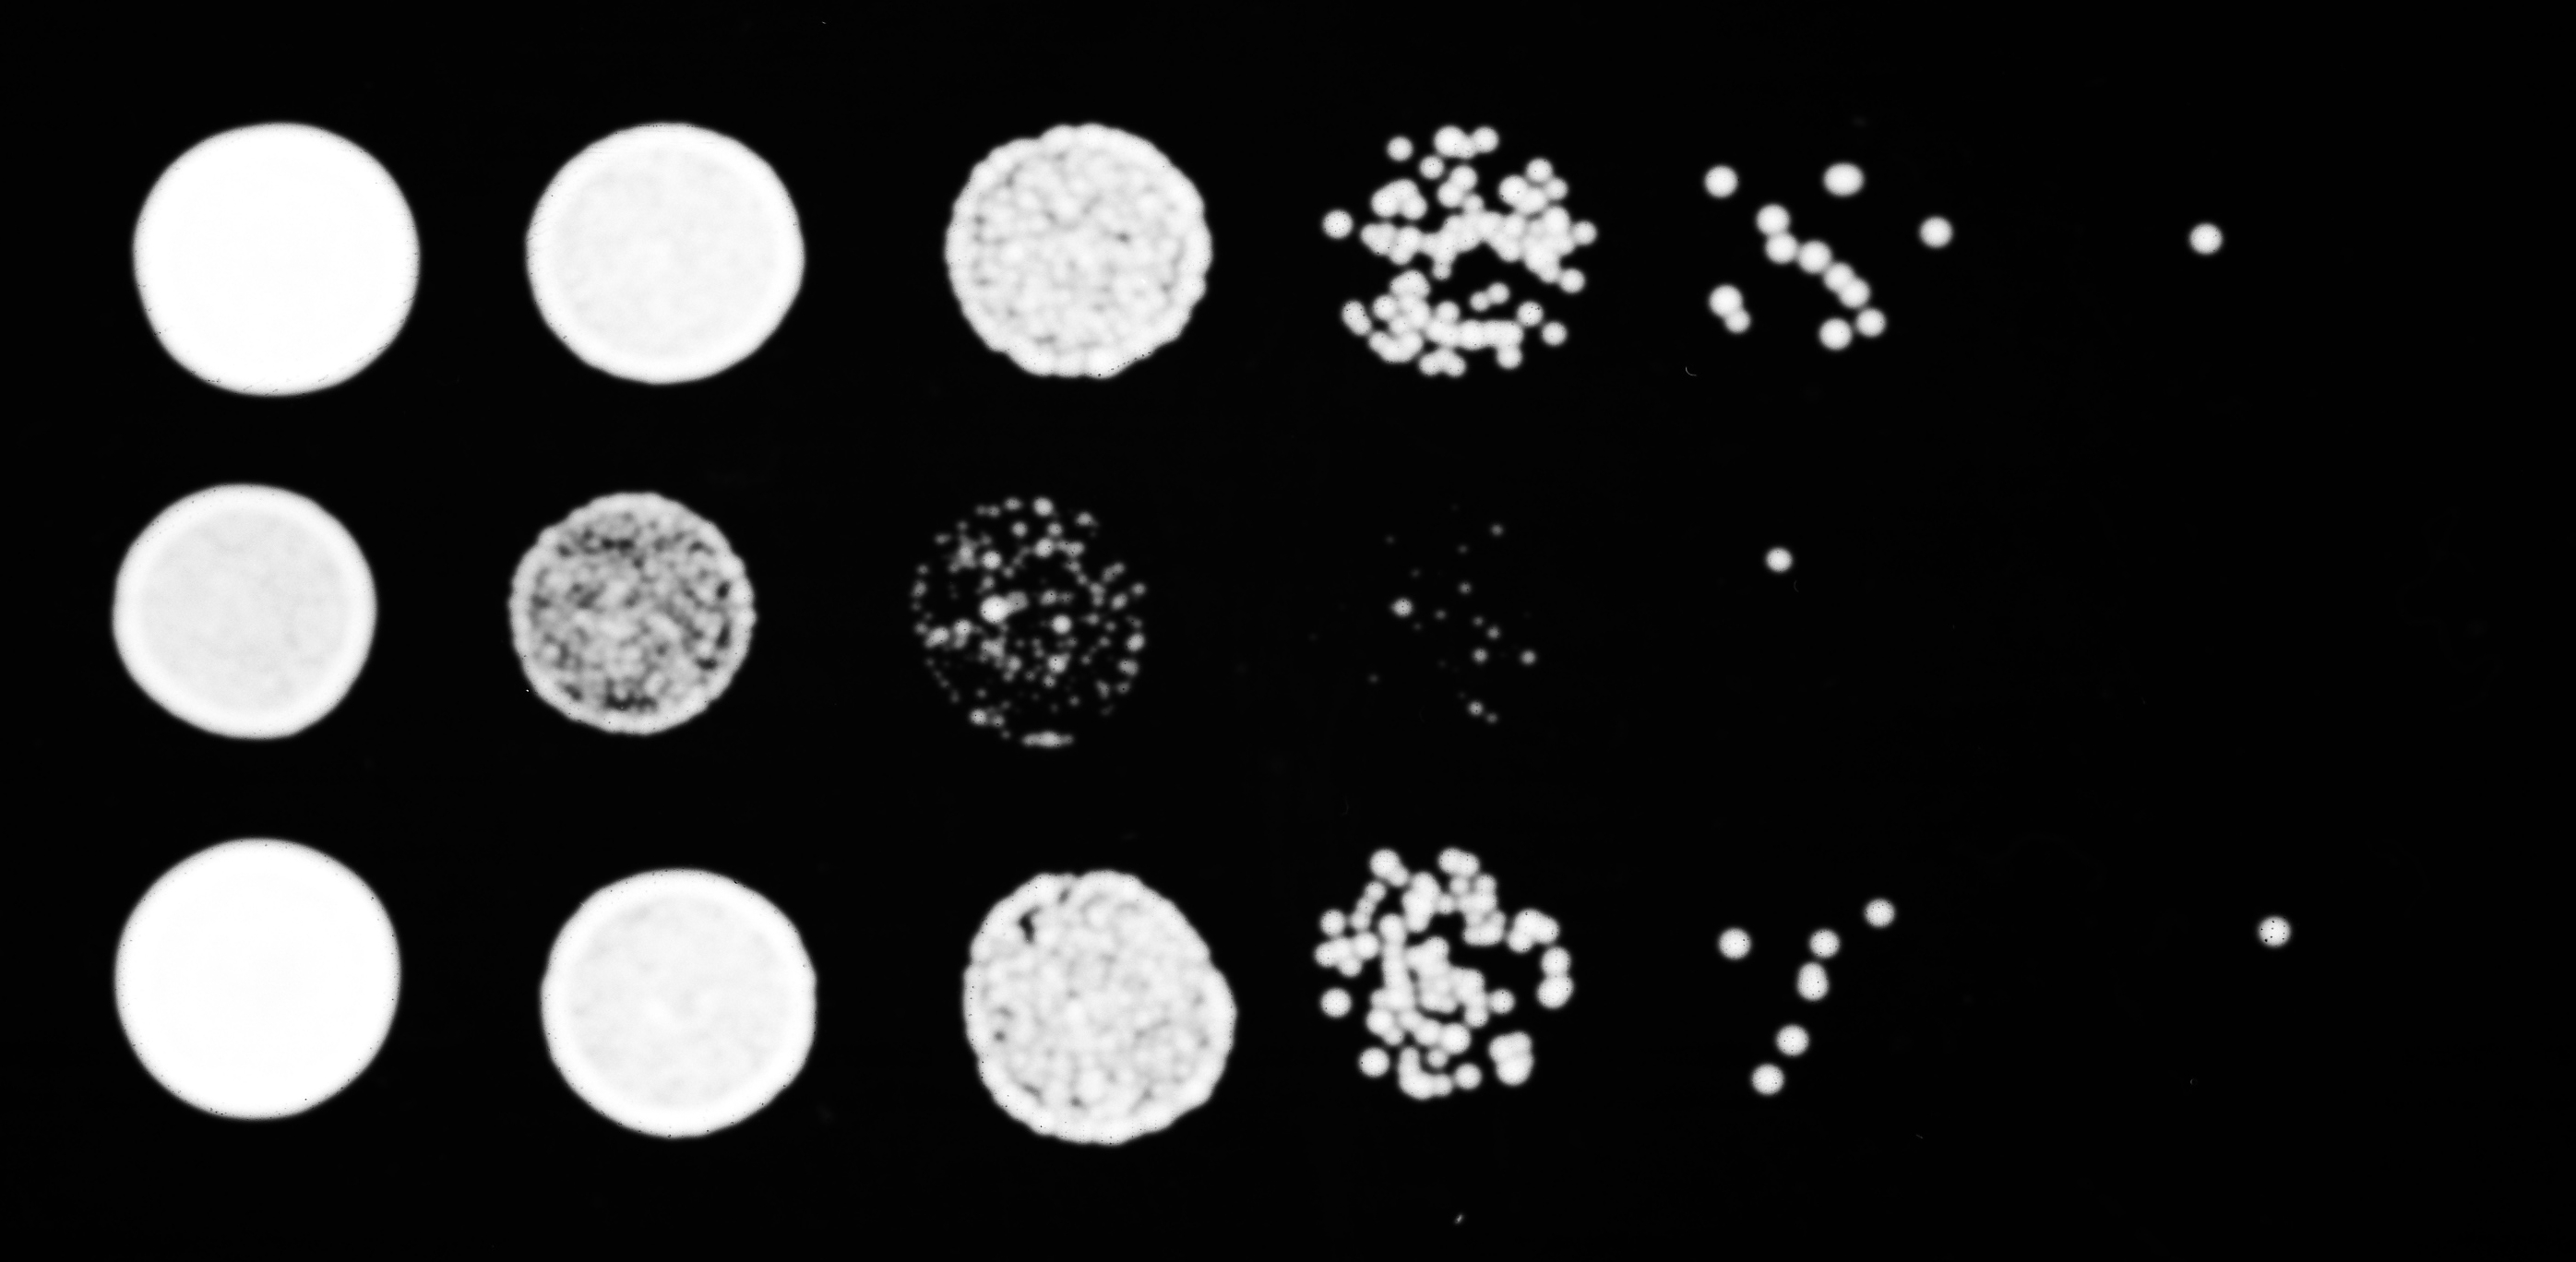
\includegraphics[width=\PicWidth]{YPE_DMSO.jpg}};
		% strains
		\pgfmathsetmacro{\Start}{0.22}
		\pgfmathsetmacro{\Sep}{0.28}
		\foreach[count=\i] \strain in {WT, \textit{arp8$\Delta$}, \textit{ino80-aa}}{
			\pgfmathsetmacro{\x}{\Start+(\i-1)*\Sep}
			\path ($(YPE.north west)!\x!(YPE.south west)$) node[xshift=-\LabelSep, anchor=east] {\strain};
		}
		%
		% YPE 37C
		\path (YPE.south) ++(0,-\VSep) node[anchor=north] (YPE_37) {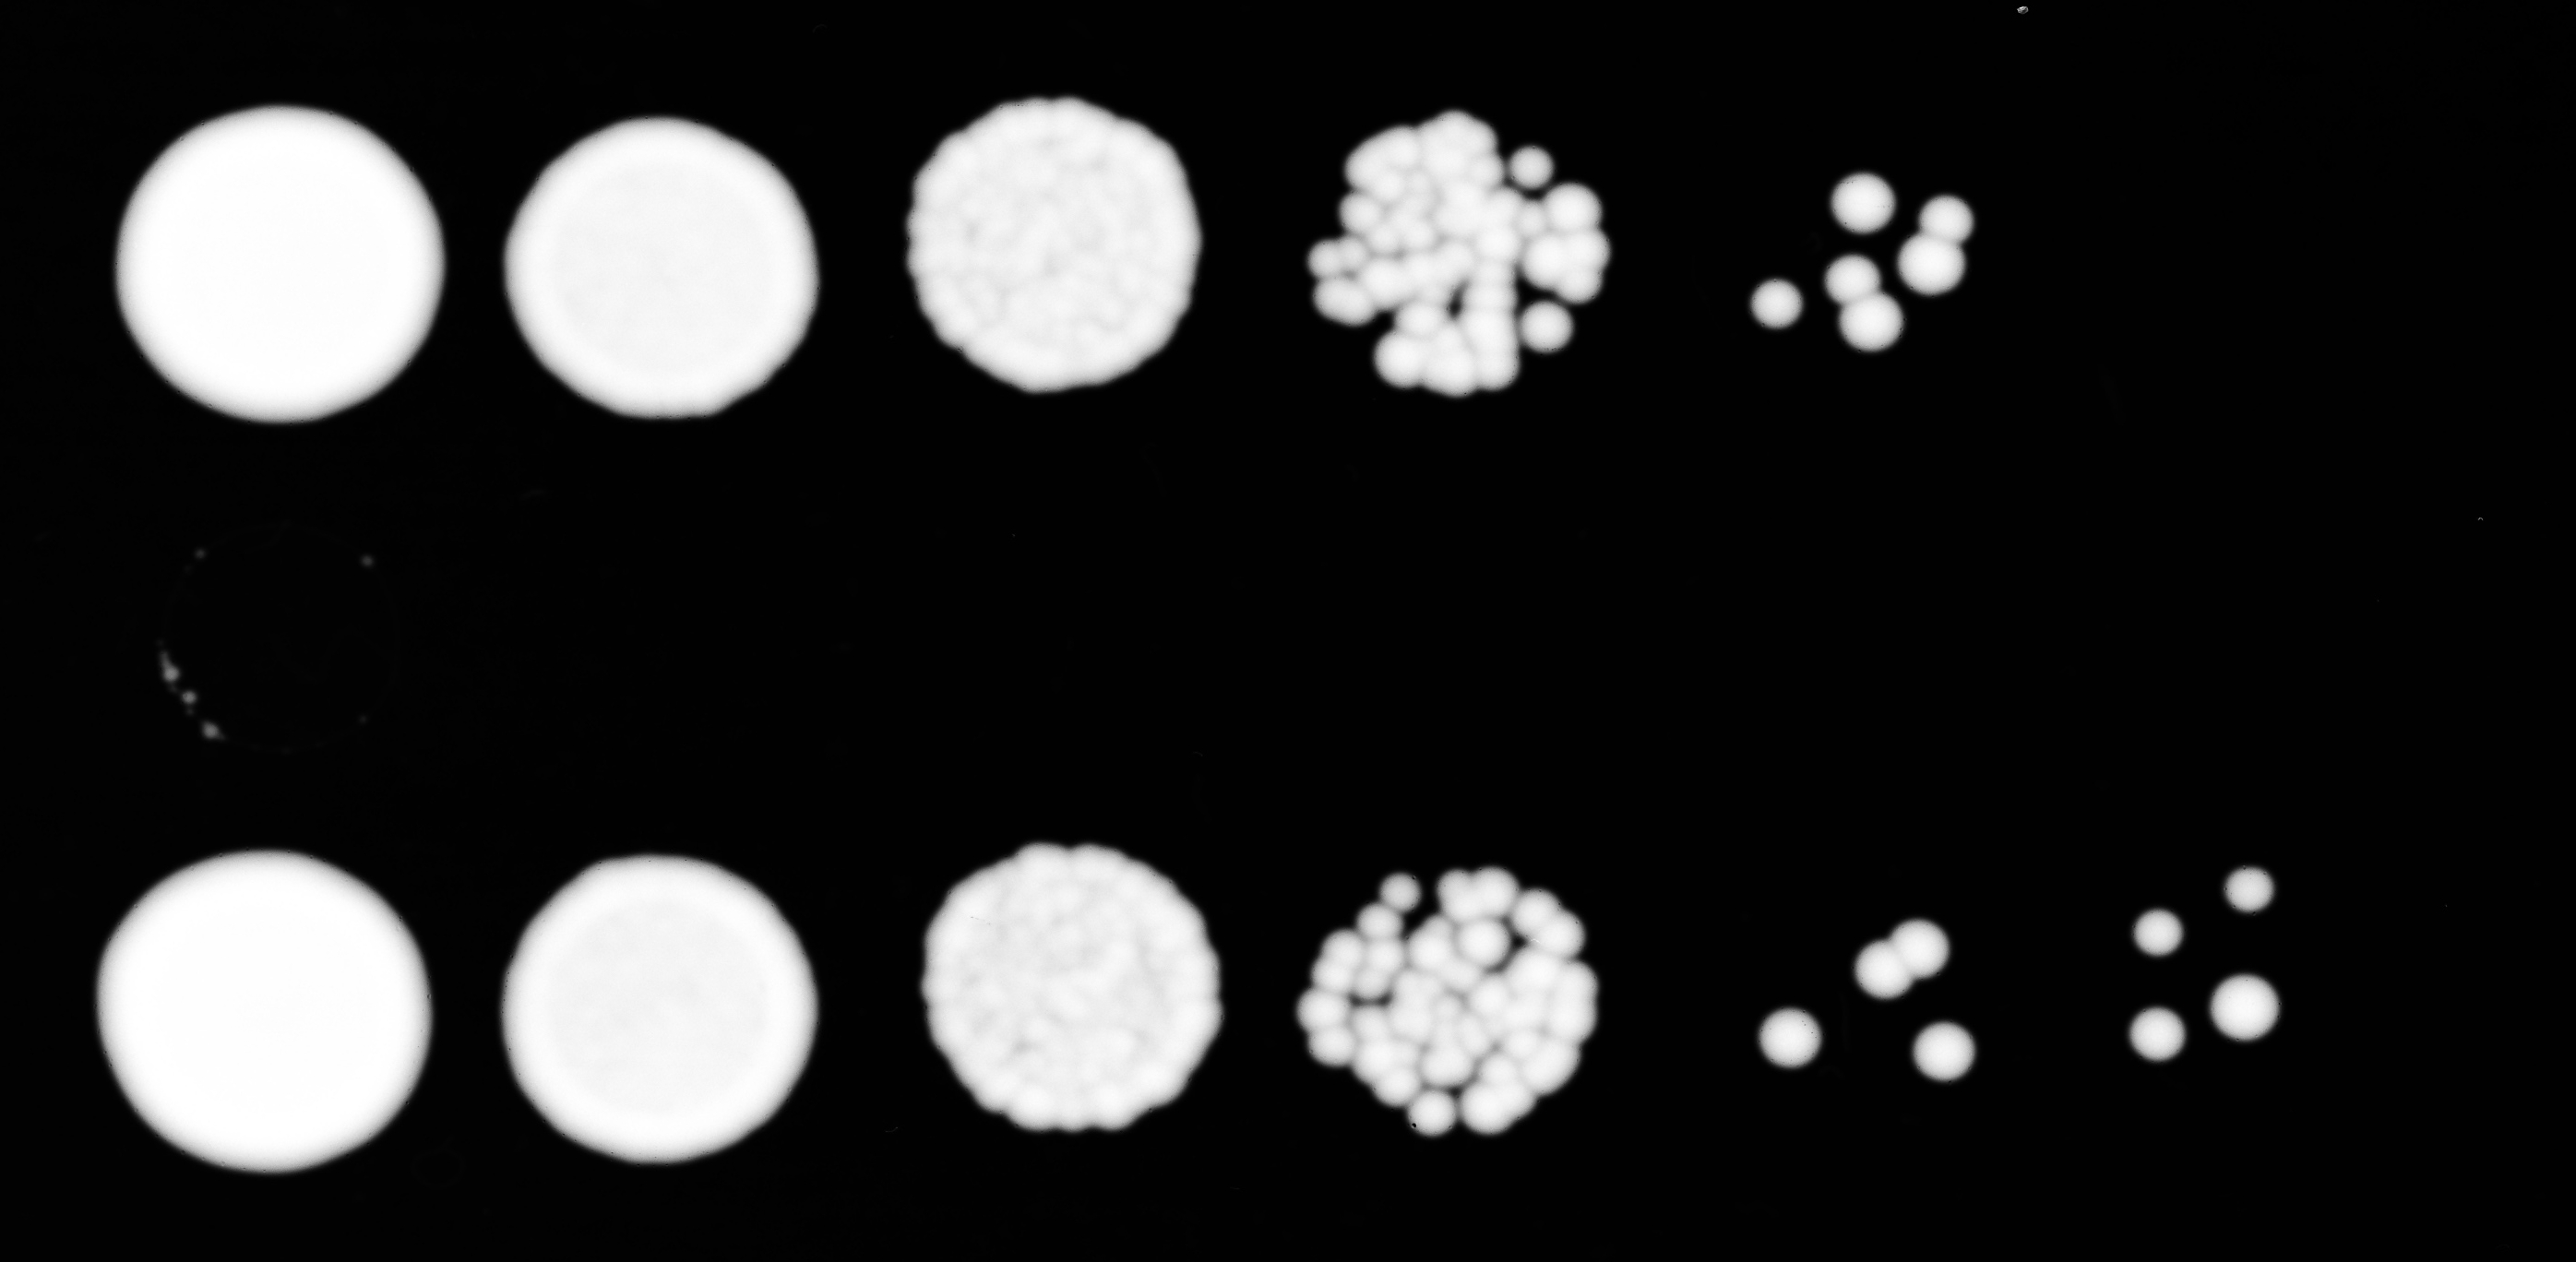
\includegraphics[width=\PicWidth]{YPE_37_DMSO.jpg}};
		% strains
		\pgfmathsetmacro{\Start}{0.22}
		\pgfmathsetmacro{\Sep}{0.28}
		\foreach[count=\i] \strain in {WT, \textit{arp8$\Delta$}, \textit{ino80-aa}}{
			\pgfmathsetmacro{\x}{\Start+(\i-1)*\Sep}
			\path ($(YPE_37.north west)!\x!(YPE_37.south west)$) node[xshift=-\LabelSep, anchor=east] {\strain};
		}
		%
		% add + Rap panels as well as sugar and strain labels
		\foreach \media/\label in {YPD/YPD, SC_wo_I/SC\\{w/o}\\Inositol,YPE/YPEthanol, YPE_37/YPEthanol\\37\textcelsius}{
			% + Rap panel
			\path (\media.east) ++(\HSep,0) node[anchor=west] (\media_Rap) {\includegraphics[width=\PicWidth]{\media_Rap.jpg}};
			%
			% sugar label
			\path (\media_Rap.east) ++(\LabelSep,0) node[anchor=west, MediaLabel] {\label};
		}
		%
		% add -/+ Rap labels
		\path (YPD.north) ++(0,\LabelSep) node[anchor=south, MediaLabel] {Mock\vphantom{p}};
		\path (YPD_Rap.north) ++(0,\LabelSep) node[anchor=south, MediaLabel] {Rapamycin};
		%
	\end{tikzpicture}
	%
\end{document}